\section{Exercise one}

Consider the following process described by the expression:
\[y(t)=e(t)+5e(t-1)\qquad e(t\sim WN(1,1))\]
The expected value of the process $y(t)$ is 6. 
\begin{enumerate}
    \item Determine the unbiased process.
    \item Find the predictor $\hat{y}(t|t-1)$. 
\end{enumerate}

\subsection*{Solution}
\begin{enumerate}
    \item The given system can be represented as:
        \begin{figure}[H]
            \centering
            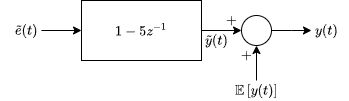
\includegraphics[width=0.5\linewidth]{images/bias.png}
        \end{figure}
        In the block diagram, we define:
        \[\begin{cases}
            \tilde{y}(t)=y(t)-m_y \\
            \tilde{e}(t)=e(t)-m_e 
        \end{cases}\rightarrow \begin{cases}
            \tilde{y}(t)=y(t)-6 \\
            \tilde{e}(t)=e(t)-1 
        \end{cases}\]
        The process $y(t)$ is composed of:
        \[y(t)=\tilde{y}(t)+6=\tilde{e}(t)\left( 1+5z^{-1} \right)+6=\left(e(t)-1\right)\left( 1+5z^{-1} \right)+6=e(t)+5e(t-1)\]
        The unbiased process is:
        \[\tilde{y}(t)=\tilde{e}(t)+5\tilde{e}(t-1)\]
        
        Since the unbiased process is not in canonical form, an all-pass filter must be used: 
        \[\tilde{y}(t)=\dfrac{1+\frac{1}{5}z^{-1}}{1}\dfrac{1+5z^{-1}}{1+\frac{1}{5}z^{-1}1}\eta(t)\]
        Here, $\eta(t)\sim WN(0,25)$. 
        
        In the time domain, this becomes: 
        \[\tilde{y}(t)=\eta(t)+\dfrac{1}{5}\eta(t-1)\]
    \item The predictor from noise is: 
        \[\hat{\tilde{y}}(t|t-1)=\dfrac{1}{5}\eta(t-1)\]
        The predictor from data is: 
        \[\hat{\tilde{y}}(t|t-1)=\dfrac{1}{5}z^{-1}\dfrac{1}{1+\frac{1}{5}z^{-1}}\tilde{y}(t)=-\dfrac{1}{5}\tilde{y}(t-1|t-2)+\dfrac{1}{5}\tilde{y}(t-1)\]
        To find the predictor of the original process by substitution, as the prediction is linear, we have:
        \begin{align*}
            &\hat{\tilde{y}}(t+1|t)=-\dfrac{1}{5}\tilde{y}(t|t-1)+\dfrac{1}{5}\tilde{y}(t) \rightarrow \\
            &\hat{y}(t+1|t)-6=-\dfrac{1}{5}\left(y(t|t-1)-6\right)+\dfrac{1}{5}\left(y(t)-6\right) \rightarrow \\
            &\hat{y}(t+1|t)-6=-\dfrac{1}{5}y(t|t-1)+\dfrac{6}{5}+\dfrac{1}{5}y(t)-\dfrac{6}{5} \rightarrow \\
            &\hat{y}(t+1|t)=-\dfrac{1}{5}y(t|t-1)+\dfrac{1}{5}y(t)+6
        \end{align*}
\end{enumerate}